\subsubsection{Interleave}
Pour essayer de diminuer les effets NUMA, nous activons la politique d'allocation mémoire interleave.
%
Les pages mémoires sont donc distribuées uniformément entre chaque banc NUMA.
%
Sur Rostand, la factorisation donne des résultats légèrement moins bons qu'avec une politique d'allocation first touch (Fig.~\ref{fig:res_facto_inter_rostand})
%
Par contre, nous obtenons une amélioration entre 3~\% et 30~\% de la résolution triangulaire pour un nombre faible de variables primaires (Fig.~\ref{fig:res_trsv_inter_rostand}).



%   (-_-)   %
\begin{figure}[!h]
     \begin{center}
        \subfigure[Factorisation ILU(0).]{%
          \label{fig:res_facto_inter_rostand}
          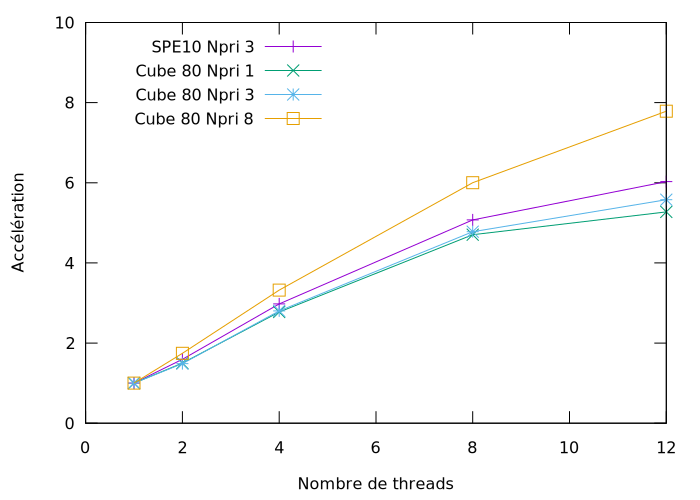
\includegraphics[width=0.49\textwidth]{res_facto_interleave}
        }%
        \subfigure[Résolution triangulaire]{%
          \label{fig:res_trsv_inter_rostand}
          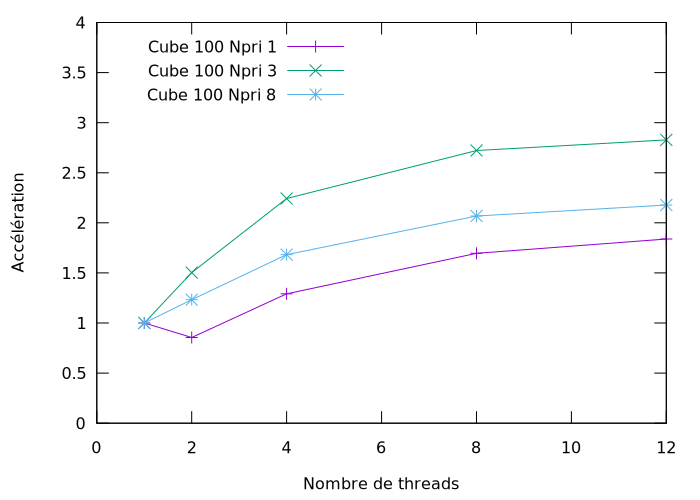
\includegraphics[width=0.49\textwidth]{res_trsv_interleave}
        }%
    \end{center}
    \caption{Performances sur Rostand en utilisant une politique d'allocation interleave.}
\end{figure}



Sur Manumanu, la factorisation se comporte de la même façon que sur Rostand (Fig.~\ref{fig:res_facto_inter_manumanu}).
%
De même, l'accélération maximale de la résolution triangulaire est meilleure avec une politique d'allocation interleave (Fig.~\ref{fig:res_trsv_inter_manumanu}).





%   (-_-)   %
\begin{figure}[!h]
     \begin{center}
        \subfigure[Factorisation ILU(0).]{%
          \label{fig:res_facto_inter_manumanu}
          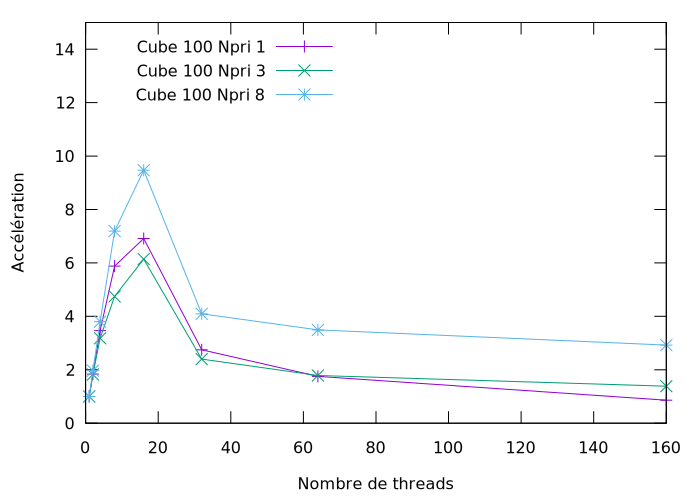
\includegraphics[width=0.49\textwidth]{res_facto_inter_manu}
        }%
        \subfigure[Résolution triangulaire]{%
          \label{fig:res_trsv_inter_manumanu}
          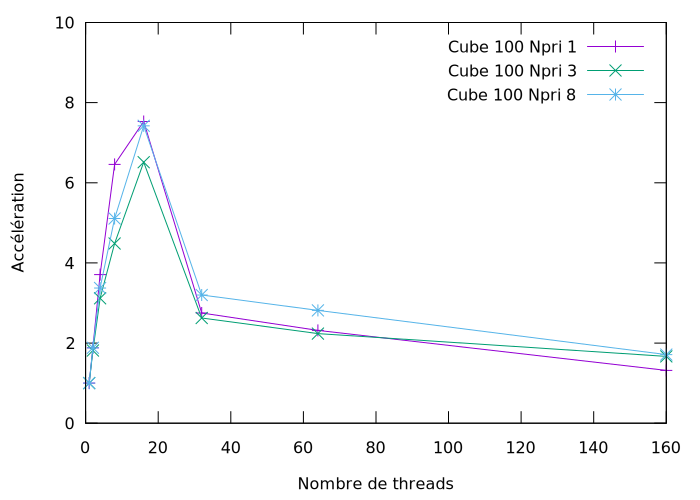
\includegraphics[width=0.49\textwidth]{res_trsv_inter_manu}
        }%
    \end{center}
    \caption{Performances sur Manumanu en utilisant une politique d'allocation interleave.}
\end{figure}
